% XeLaTeX can use any Mac OS X font. See the setromanfont command below.
% Input to XeLaTeX is full Unicode, so Unicode characters can be typed directly into the source.

% The next lines tell TeXShop to typeset with xelatex, and to open and save the source with Unicode encoding.

%!TEX TS-program = xelatex
%!TEX encoding = UTF-8 Unicode

\documentclass[12pt,oneside,a4paper]{report}
\usepackage[bookmarks=true, bookmarksopen=true, colorlinks=false, linkcolor=black, driverfallback=dvipdfm, pdfstartview=FitH, hidelinks]{hyperref}	%在PDF中增加Bookmaker

\usepackage{color}
\definecolor{bisque}{rgb}{.996,.891,.755}

% 設定頁面留白寬度(gene 2.5cm 可改成1cm)
\usepackage[top=2.5cm,bottom=2.75cm,left=2.5cm,right=2.5cm]{geometry}   %設定頁面留白

\usepackage[boldfont,slantfont,CJKnumber,CJKspace]{xeCJK}	%xeCJK套件
\usepackage{CJKnumb}
\setmainfont{Times New Roman}								%設定英文預設字體
\setCJKmainfont{標楷體}                                      %設定中文預設字體
\setCJKsansfont{標楷體}
% \setCJKmainfont{cwTeX Q Kai Medium}                       %若標楷體無法使用之中文預設字體
% \setCJKsansfont{cwTeX Q Kai Medium}

\usepackage{eso-pic}										%插入浮水印
\usepackage{graphicx}										%插入圖片
\usepackage[bf,indentfirst,pagestyles]{titlesec}			%定義章節名稱與文字型態
\usepackage{titletoc}										%定義章節名稱
\usepackage{cite}											%bibliography package
\usepackage{tabularx}
\usepackage{longtable}										%處理長表格
\usepackage{enumitem}
\usepackage{array}
\usepackage{float}
\usepackage{fancyvrb}
\usepackage{fancyhdr}
\usepackage[above]{placeins}
\usepackage{pstricks,pst-node,pst-tree}
\usepackage{wrapfig}
\usepackage{graphicx}
\graphicspath{ {./img/} }
\usepackage{caption}
\usepackage{subcaption}
\usepackage{multirow}
\usepackage{url}
\usepackage{listings}
\usepackage{color}
\usepackage{pdfpages}

\definecolor{light-gray}{gray}{0.95}

\lstset{
    basicstyle=\linespread{1.0}\ttfamily\footnotesize,
    backgroundcolor=\color{light-gray}, 
    xleftmargin=0.7cm,
    frame=tlbr, 
    framesep=0.2cm, 
    framerule=0pt,
}
\setbox0=\hbox{\ttfamily}

%定義環境變數與巨集指令
%-------------------基本設定------------------------------------%
% 沿用 latex 的一些標點的轉換,如 en-dash 以兩個減號表示
\defaultfontfeatures{Mapping=tex-text}
\XeTeXlinebreaklocale "zh"
\XeTeXlinebreakskip = 0pt plus 1pt
%-------------------------------------------------------------%

%-------------------重新定義章節名稱格式--------------------------%
\titleformat{\chapter}[hang]{\centering\huge\bfseries}{第\CJKnumber{\thechapter}章}{1em}{}
%\renewcommand\chaptername{Chapter\hspace{.5em}\thechapter}
\renewcommand\contentsname{目錄}
\renewcommand\listfigurename{圖目錄}
\renewcommand\listtablename{表目錄}
\renewcommand\lstlistlistingname{程式碼目錄}
\newcommand{\loflabel}{圖} % 定義圖目錄顯示方式
\newcommand{\lotlabel}{表} % 定義表目錄顯示方式
\newcommand{\loclabel}{程式碼}

\titlecontents{chapter}[0pt]{}
    {第\CJKnumber{\thecontentslabel}章\quad}{}
    {\hspace{.5em}\titlerule*[10pt]{$\cdot$}\contentspage}
\titlecontents{section}[2em]{}
    {\thecontentslabel\quad}{}
    {\hspace{.5em}\titlerule*[10pt]{$\cdot$}\contentspage}
\titlecontents{subsection}[4em]{}
    {\thecontentslabel\quad}{}
    {\hspace{.5em}\titlerule*[10pt]{$\cdot$}\contentspage}

\renewcommand{\bibname}{參考文獻}            %修改參考文獻的標題名
\titlespacing{\chapter}{0pt}{*0}{*4}        %設定標題與四周的距離
\titlelabel{\thetitle\quad}				    %設定章節標題的樣式
\renewcommand{\figurename}{圖}
\renewcommand{\tablename}{表}
\renewcommand{\lstlistingname}{程式碼}
%-----------------------------------------------------------------%

%-------------------設定行距--------------------------------------%
\renewcommand{\baselinestretch}{2.1} % 大約等於word1.5倍行高

%設定enumerate等的item間距
\usepackage{enumitem}
\setenumerate{itemsep=-5pt}
\setitemize{itemsep=-5pt}
\setdescription{itemsep=-5pt}
%-----------------------------------------------------------------%

%-------------------定義浮水印------------------------------------%
\newcommand\WatermarkPicture{
   \put(0,0){
   \parbox[b][\paperheight]{\paperwidth}{
     \vfill
     \centering
     
\includegraphics[width=12.75cm,keepaspectratio]{watermark_ntut.png}%
     \vfill
     }
   }
}
%-----------------------------------------------------------------%

%------------------圖片巨集---------------------------------------%

%巨集格式
%mygraphic{圖片KeyWord}{圖片註解}{圖片路徑}
\def\myGraphic#1#2#3
{
	\begin{figure}[!htbp]
		\begin{center}
			\includegraphics[width=\textwidth]{#3}
			\caption{#2}\label{#1}
		\end{center}

	\end{figure}
}
%-----------------------------------------------------------------%

%------------------小小圖片巨集---------------------------------------%

%巨集格式
%mygraphic{圖片KeyWord}{圖片註解}{圖片路徑}
\def\myGraphicSS#1#2#3
{
	\begin{figure}[!htbp]
		\begin{center}
			\includegraphics[width=2cm]{#3}
			\caption{#2}\label{#1}
		\end{center}

	\end{figure}
}
%-----------------------------------------------------------------%

%------------------小圖片巨集---------------------------------------%

%巨集格式
%mygraphic{圖片KeyWord}{圖片註解}{圖片路徑}
\def\myGraphicS#1#2#3
{
	\begin{figure}[!htbp]
		\begin{center}
			\includegraphics[width=6cm]{#3}
			\caption{#2}\label{#1}
		\end{center}

	\end{figure}
}
%-----------------------------------------------------------------%

%------------------中圖片巨集---------------------------------------%

%巨集格式
%mygraphic{圖片KeyWord}{圖片註解}{圖片路徑}
\def\myGraphicM#1#2#3
{
	\begin{figure}[!htbp]
		\begin{center}
			\includegraphics[width=8cm]{#3}
			\caption{#2}\label{#1}
		\end{center}

	\end{figure}
}
%-----------------------------------------------------------------%

%------------------大圖片巨集---------------------------------------%

%巨集格式
%mygraphic{圖片KeyWord}{圖片註解}{圖片路徑}
\def\myGraphicB#1#2#3
{
	\begin{figure}[!htbp]
		\begin{center}
			\includegraphics[width=12cm]{#3}
			\caption{#2}\label{#1}
		\end{center}

	\end{figure}
}
%-----------------------------------------------------------------%

%------------------大大圖片巨集---------------------------------------%

%巨集格式
%mygraphic{圖片KeyWord}{圖片註解}{圖片路徑}
\def\myGraphicBB#1#2#3
{
	\begin{figure}[!htbp]
		\begin{center}
			\includegraphics[width=16cm]{#3}
			\caption{#2}\label{#1}
		\end{center}

	\end{figure}
}
%-----------------------------------------------------------------%

%------------------表格巨集---------------------------------------%
\renewcommand{\arraystretch}{1}

%巨集格式
%myTable{Table KeyWord}{Table註解}
\def\myTable#1#2
{
	\begin{table}[!htbp]
	\setlength{\abovecaptionskip}{0pt}
	\setlength{\belowcaptionskip}{10pt}
	\begin{center}
	\caption{#2}\label{#1}
}


\def\endmyTable
{
	\end{center}
	\end{table}
}

%-----------------------------------------------------------------%

%------------------修改圖與表的註解編號格式-----------------------%

\makeatletter
\long\def\@makecaption#1#2{%
  \vskip\abovecaptionskip
  \sbox\@tempboxa{{#1}\quad #2}%
  \ifdim \wd\@tempboxa >\hsize
    {#1}\quad #2\par
  \else
    \global \@minipagefalse
    \hb@xt@\hsize{\hfil\box\@tempboxa\hfil}%
  \fi
  \vskip\belowcaptionskip}
\makeatother

%-----------------------------------------------------------------%
%------------------修改Description縮排格式--------------------------%
%\makeatletter
%\renewenvironment{description}
%  {\list{}{\leftmargin\z@ \labelwidth\z@ \itemindent-\leftmargin
%   \let\makelabel\descriptionlabel}}
%  {\endlist}
%\makeatother
%-----------------------------------------------------------------%
%------------------Use Case巨集---------------------------------------%
%巨集格式
%useCase{UseCase名稱}{UseCase圖片路徑}
\def\useCase#1#2#3
{
	\subsection{#1}
	\begin{figure}[!htb]
		\begin{center}
			\includegraphics[width=\textwidth]{#2}
		\end{center}
	\end{figure}
}
% \graphicspath{{./picture/eps/}{./picture/png/}}
% \graphicspath{{.}}					%告訴Latex去這兩個目錄下找圖檔
%-----------------------------------------------------------------%
%-------------------為了方便所設定的巨集--------------------------%

%-----------------------------------------------------------------%


\begin{document}
\includepdf[pages={1}]{bookname_front_and_back_covers.pdf}
\includepdf[pages={2}]{bookname_front_and_back_covers.pdf}

\includepdf[pages={1}]{bookname.pdf}

\AddToShipoutPicture{\WatermarkPicture}                     % 加入浮水印

\pagenumbering{roman} 										%論文篇前之頁數為羅馬數字
\chapter*{摘~~要}
\addcontentsline{toc}{chapter}{中文摘要}

%基本資訊

\noindent
論文名稱:一個提高判斷HTML中元件差異速度的瀏覽器擴充套件\\
頁數:XX頁\\
校所別:國立台北科技大學~資訊工程系碩士班\\
畢業時間:一百一十學年度第二學期\\
學位:碩士\\
研究生:廖昱翔\\
指導教授:陳碩漢教授\\
\hspace*{\fill}\\
\noindent
關鍵字:HTML、自動化驗收測試、瀏覽器擴充套件、比較HTML內容\\
\hspace*{\fill}\\
%
\indent
在自動化網頁測試中,會一直運用到Xpath表達式來定位在HTML文本中元件的位置。在一個大型的HTML文本中,時常會透過和網站元件的互動,從而來改變HTML的屬性或資料。一個測試人員在撰寫自動化腳本的時候,可能只會專注在單一元件屬性的變化,而較困難去找出其他更適合可以拿來當作限制條件的元素

本論文提出利用文本比較的方式加在瀏覽器Developer tools上做成一個擴充套件,除了可以在元件旁邊的頁面下看到當前節點和先前節點的比較,以及可以在主頁面下看到HTML文本所有的比較結果,另外加入了倒數計時功能,可以在不用點擊觸發比較的情況下,產生出結果,讓開發者可以根據結果來縮減Xpath長度以及耐用度,進而增加程式提升穩定性。										%中文摘要
\chapter*{ABSTRACT}
\addcontentsline{toc}{chapter}{ABSTRACT}

%基本資訊

\noindent
Title:Facilitating The Process Rate Of Difference Determination Within HTML After Events Triggered In Web Page\\
Pages: XX\\  %待修正
School: National Taipei University of Technology\\
Department: Computer Science and Information Engineering\\
Time: July,2022\\
Degree: Master\\
Researcher: LIAO,YU-SIANG\\
Advisor: XXX %待修正
\hspace*{\fill}\\
Keywords: Automated acceptance tests, Browser extension tool, Compare HTML content \\
\hspace*{\fill}\\
\indent %待修正

Writing automated web testing scripts mainly uses programs to simulate the situation of users operating web pages.
In order to determine whether the interactive components in the website are normally triggered, 
a part of change HTML content will be used as the judgment condition for the success of the interaction.
Testers make it difficult to find stable element constraints in more efficient way 
because components change rapidly or only focus on the current component changes.

This thesis proposes to use the HTML text comparison method to develop an browser extension package 
that use in the browser developer tools.
Testers can get all the differences in the panel of browser developer tools if detail of the element is changed because of interactive components.
In order to maintain HTML content after interacting and reduce unnecessary compared result, we designed with timing and filtering functions additionally.

The three major functions of the extension will allow developers to reduce the Xpath length 
and durability according to the results, thereby increasing the program stability.										%英文摘要
\chapter*{誌~謝~}
\addcontentsline{toc}{chapter}{誌謝}

\indent
 首先要感謝我的指導教授謝金雲老師和鄭有進老師,在這兩年內辛苦的指導,讓我在這些時間內學習到眾多的專業知識與技能,並且讓我有機會擁有一個大型軟體專案開發的經驗,也十分感謝口試委員劉立頌老師、陳碩漢老師,對於我的論文提出十分多的建議,讓我的論文能夠更加完整並且對於研究室內的團隊有所貢獻。

\indent
 此外十分感謝研究室內的同學們、學長們、學弟妹們,在我寫論文的過程中給予我很多幫助,並且協助我完成論文所需的實驗,以及兩年內所有的陪伴,有你們在的研究室永遠是最愉快的。

\indent
 最後感謝我的家人們對於我在台北讀研究所時,不斷的關心以及關懷,真的非常感謝你們的支持與關心,還有我的女友安安,在我忙碌的時候耐心的陪伴我、鼓勵我,讓我知道我不是一個人在面對這一切,並且順利取得碩士學位。											%誌謝
\newpage

\addcontentsline{toc}{chapter}{目錄}
\tableofcontents 											%引入目錄
\newpage

\addcontentsline{toc}{chapter}{表目錄}
\renewcommand{\numberline}[1]{\lotlabel~#1\hspace*{1em}}
\listoftables												%引入表目錄
\newpage

\addcontentsline{toc}{chapter}{圖目錄}
\renewcommand{\numberline}[1]{\loflabel~#1\hspace*{1em}}
\listoffigures												%引入圖目錄
\newpage													%換新頁


\addcontentsline{toc}{chapter}{程式碼目錄}
\renewcommand{\numberline}[1]{\loclabel~#1\hspace*{1em}}
\lstlistoflistings
\newpage

\pagenumbering{arabic}										%論文內文之頁數為阿拉伯數字

\chapter{緒論}
\section{研究背景與動機}
\indent
Robot Framework\cite{robotframework}是一個自動化測試框架,其中的關鍵字可被視為一個測試步驟,透過將多個關鍵字包裹成一個更高層級的關鍵字時,便可將其視為一個測試流程。

\indent
當多個團隊一起開發測試腳本時,關鍵字能夠盡量被重複使用是一個常見的目標。而部份情況中我們可以在撰寫測試腳本時就判斷出撰寫的測試步驟是可以被重複使用,因而將其提前包裹成一個新關鍵字,例如當我們在同一個測試腳本中,有多個步驟需要重複使用時,我們便會提前將其抽取成一個關鍵字提供多處使用,這是可以預知的;但大部分的情況中,我們無法預期目前所撰寫的測試步驟是否會被其他測試腳本再次使用,以兩個測試團隊為例:其中一個測試團隊需要以創立一個項目的流程作為測試腳本中的主要步驟,另外一個測試團隊也需要相同的流程做為測試資料的準備,平時撰寫測試腳本時,兩個組別無法隨時互相溝通,只能以現有的情況做為判斷,因此無法透過提前判斷而去抽取成一個關鍵字,或者其中一個團隊剛好發現其他團隊已有撰寫好之流程,直接拿取做使用且當下未立刻進行抽取關鍵字之重構,導致後續時常需要對現有的程式碼進行重構。

\indent
進行重構時,重複的測試步驟往往都是存在於不同的檔案中,一不小心就會有部分程式碼未修改,直到後續執行時才發現錯誤,這些經常都是人為錯漏所導致的。為了避免以上所提及的錯誤不斷發生,導致測試團隊必須再次花費時間針對缺漏的錯誤進行修正,因此在測試團隊重構時,需要一個能夠避免人為錯漏且更加方便的重構工具。

\section{研究目標}
\indent
劉冠志論文\cite{LIU-Thesis}中提供了測試腳本重構工具RF Refactoring,此工具提供了三種Robot Framework測試腳本的重構方法,分別為重新命名關鍵字、重新命名變數,以及修改關鍵字介面,但仍然無法解決目前所遭遇之問題,因此本論文將針對此工具進行改善,否則開發人員只能使用目前用來撰寫Robot Framework測試腳本的整合式開發環境(RED\cite{RED}、Visual Studio Code\cite{VSCode})中的搜尋取代工具進行重構,因而造成重構效率的降低,以及人工檢查的疏忽,導致重構的錯誤和缺漏等等。為此工具增加重構方法之多元選擇,使其可根據測試人員的需求重構測試腳本,並且在重構過程中能夠避免人為錯漏的問題發生。

\section{論文組織架構}
\indent
本論文共有六章節,第二章將介紹背景知識及使用工具,第三章介紹擴充RF Refactoring之方法設計,其中介紹了欲擴充之重構方法及其流程,並且介紹如何將重構方法擴充至RF Refactoring中,第四章將會以第三章所設計之方法進行實作,其中包含了重構流程及外掛程式之實作,第五章將以實際Robot Framework測試腳本介紹重構案例,並且邀請測試團隊成員分別使用Visual Studio Code搜尋取代工具及本論文擴充後之重構工具進行重構,後續比較使用之差異。
\chapter{背景知識}

\section{HyperText Markup Language(HTML)}\label{s2.1}
\indent
標記式語言(Markup Lanaguage)\cite{HTML}是一種利用電腦看得懂的標示符號來定義出一份資料會如何呈現在畫面中,
而超文本標記語言(HyperText Markup Language),簡稱HTML,則是用於建立網站的標記式語言,
透過網頁瀏覽器的讀取,可以將其轉換成視覺化的網站。
雖然它不算是程式語言的一種,卻是架構網站的重要根基。

\begin{figure}[H]
    \centering
    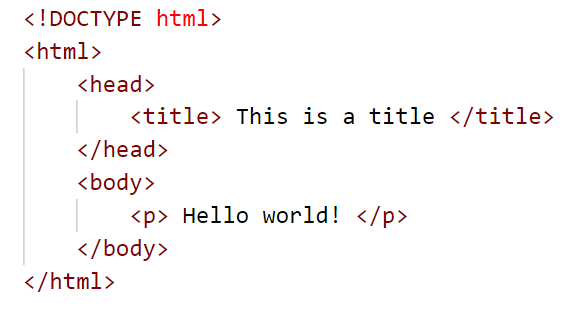
\includegraphics[width=0.55\textwidth]{picture/ch2-htmlExample.png}
    \caption{HTML檔案範例}
    \label{f2.1}
\end{figure}

\section{Node.js}\label{s2.2}
Node.js\cite{Node.js}是一個能夠在伺服器端執行JavaScript的Open Source跨平台執行環境,讓JavaScript這種程式語言不僅僅只能在操作使用者端的程式碼。
它是讓使用者把僅能在瀏覽器執行JavaScript的限制,改成可以透過電腦中的終端介面來直接執行JavaScript程式碼。
而node.js是一個輕量的framework,它裡面的每個JavaScript檔案都會被視為一個module,使用者可以用可下載的或可自己撰寫的模組來實現自己想要的功能。

\subsection{cherrio}\label{s2.2.1}
cherrio是在Node.js的一個模塊,實現了把jQuery中Selector輕量化的功能,需要先讀入HTML進行解析,並使用選擇器找出所需要的元件節點來作客置化的操作。
例如:若需要進行爬蟲的話,需要先讀入一整個完整的網頁HTML,並利用元件的條件來找出該元件來讀出該文字內容。

\subsection{Diff}\label{s2.2.2}
Diff是在Node.js的一個模塊,本論文取用的Hiff開源程式庫\cite{Hiff}是以該模塊為基礎而開發的,
利用其中的API來做兩個參數中的比較並顯出是否有差異,參數的類型可以是字元陣列...等等不同類別。

\section{DOM-based Locators}\label{s2.3}
如果要去抓取網頁其中一個物件,並使我們可以透過程式對它進行各式各樣的操作,
方法基本上可以分類成三種\cite{Web-Locators}:

\indent
1. Coordinate-based locators: 使用座標定位。

\indent
2. DOM(Document Object Model)-based locators: 使用文件物件模型(DOM)定位。

\indent
3. Visual locators: 使用視覺定位,通常使用影像辨識技術。

\indent
本論文中談論的情境是以穩定性較高的DOM-based locators來操作其中的物件,其中DOM在此指的是網頁中的樹狀結構HTML文件結構。
而利用此定位實現的技術即為XPath (XML Path Language)\cite{Xpath}。

\section{XML Path Language (XPath)}\label{s2.4}
XML Path Language (XPath) 是一種用來尋找XML文件中一個或多個節點位置的查詢語言。
以XML中樹狀結構為基礎,
讓使用者用一個附帶多個條件的表達式,
找到是否有符合這些條件的路徑,
通常程式使用介面是由HTML構成的,
而HTML結構屬於XML結構的一種,
所以在網頁自動化測試中經常使用XPath定位找出元件位置\cite{Test-Case-Aging-By-Xpath}並對該元件進行操作。。


在Xpath表達式中,最常見的是路徑表達式\cite{Xpath-Selenium-Selectors}。
路徑表達式是從一個XML節點到另一個節點或一組節點的步驟順序。
如下圖表示,從HTML起始節點「ul」到屬性id為second-level的節點「li」,再從節點「li」到節點「div」,
其路徑表達式為\colorbox{lightgray}{/ul/li[@id="second-level"]/div}                                                                                                                                                                                                                                                   

\begin{figure}[H]
    \centering
    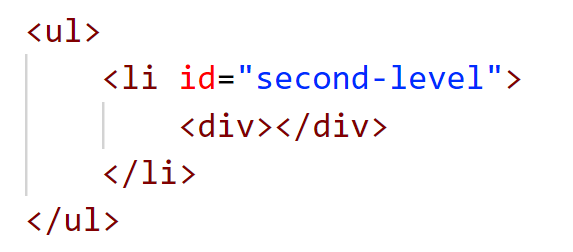
\includegraphics[width=0.5\textwidth]{picture/ch2-xpathExample.png}
    \caption{HTML檔案範例}
    \label{f2.2}
\end{figure}

路徑表達式通常由三個元件設定來組成的,
以圖\ref{f2.2}的路徑表達式為例:

\begin{itemize}
\item[●] 一個 Axis。代表搜尋的方向,例如:路徑表達式中的\colorbox{lightgray}{/}
\item[●] 一個 Node test。可以選擇指定或不指定特定的 HTML 的標籤名稱,例如表達式中的\colorbox{lightgray}{li}
\item[●] 零個或多個 Predicate。描述搜尋節點的條件,藉此可以過濾出需要的節點,例如:\colorbox{lightgray}{/li[@id="second-level"]}
\end{itemize}

\section{Chrome Developer Tools}\label{s2.5}
基於桌機瀏覽器市占排行,本論文選用市佔率第一個Chrome使用。
在瀏覽器的頁面中,可以點擊功能鍵F12,即可打開Chrome Developer Tools\cite{Chrome-Developer-Tools}。
本工具最常用的四個功能模塊為:
\begin{itemize}
    \item[●] 元素(Elements):主要可以展示出該網站的當下HTML檔,以及每個元素對應的CSS屬性...等等細部設定,也可以及時修改當下的檔案,查看若更改會有什麼情況。
    \item[●] 控制台(Console):類似作業系統中的命令提示字元,可以在以網頁的形式讓電腦傳遞給我們一些資訊,例如:輸入Xpath查看是否有定位到該物件以及程式中若需要輸出字元字串,則會在這個頁面下呈現...等等功能。
    \item[●] 源代碼(Sources):從該頁面可以知道該網站的HTML、Javascrpit和CSS...等等程式,也可以從這裡設定斷點,來增加Debug的效率。
    \item[●] 網路(Network):在網站運行時,可以透過該頁面觀察此網頁和伺服器傳遞Request的情況,也可以手動調整網路的速度來檢測網站的穩定性。
\end{itemize}

\begin{figure}[H]
    \centering
    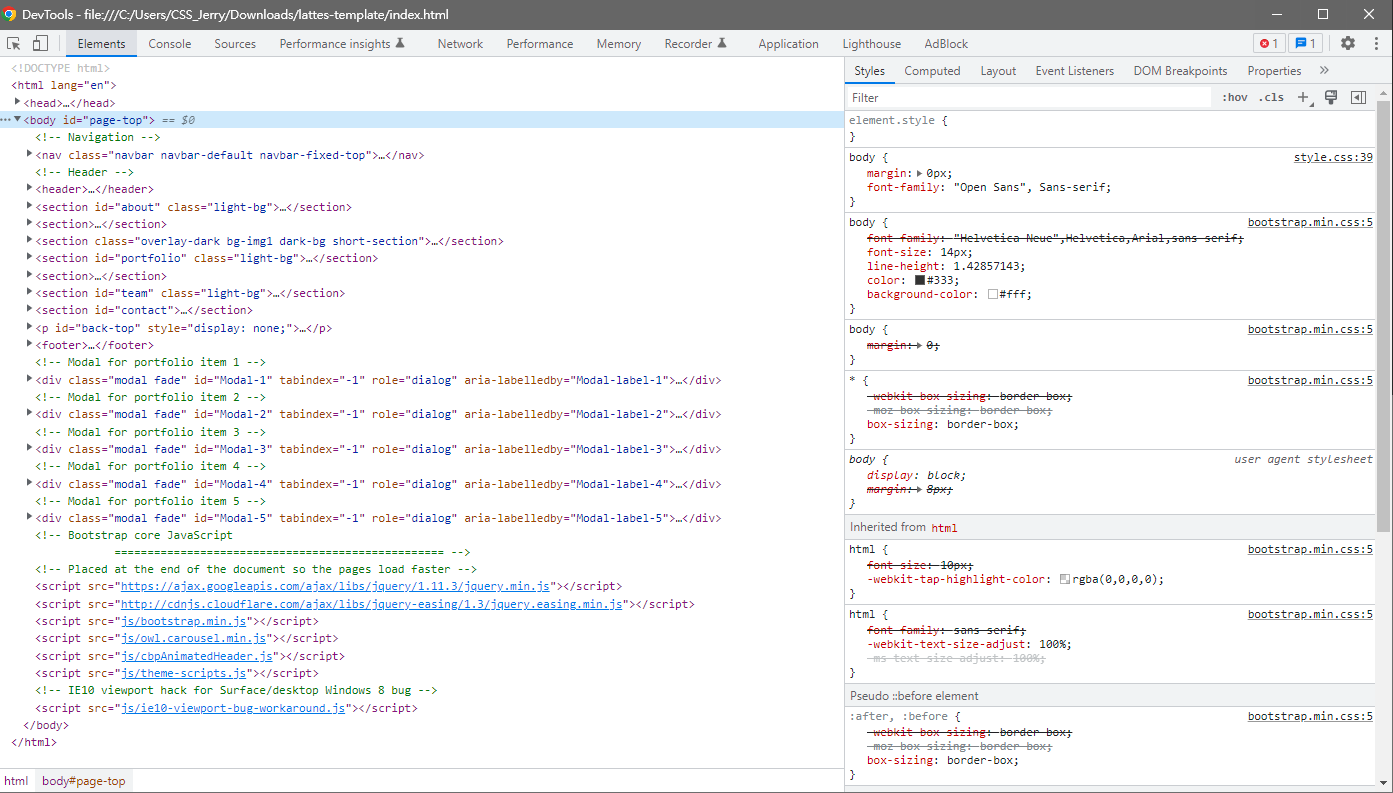
\includegraphics[width=0.8\textwidth]{picture/ch2-chromeDeveloperTool.png}
    \caption{Chrome Developer Tool頁面範例}
    \label{f2.3}
\end{figure}

\section{Chrome Extension}\label{s2.6}

瀏覽器除了有本身基本的功能之外,如果使用者還有其他需求的話,可以去網路商城下載擴充套件或自己撰寫相關程式來讓瀏覽器可以達到使用者額外的需求。
一般來說擴充元件\cite{Chrome-Extension}\cite{Chrome-Extension-Thesis}都是用諸如HTML、CSS和JavaScript的網路技術,另外有些還會透過瀏覽器的API來做溝通及變換畫面。
例如:目前市面上有很多人使用網頁版的Google翻譯來解決一般人難以讀懂英文文章的困擾,
但每次都需要跳轉到網頁才可以翻譯,
Google翻譯擴充套件能讓使用者在當下的畫面把文字圈選起來,利用程式判斷出圈起來文字並進行翻譯,
最後在該頁面的HTML增添一些元件來顯示出翻譯的結果供讀者參考。

\subsection{輸入元件}\label{s2.6.1}
Chrome瀏覽器提供能讓使用者和網頁互動的元件,有畫面可見的瀏覽器按鈕和網頁中內容...等等UI元素,也有畫面中的右鍵功能選單和快捷鍵...等等被隱藏的區塊。

\subsection{安裝檔Manifest.josn}\label{s2.6.2}
作為擴充元件的安裝檔,內部記錄了很多很多重要的程式路徑以及權限設定...等等的相關資訊,
若需要將此擴充元件安裝在瀏覽器中使用,需要透過載入此檔案,讓瀏覽器可以支援此程式包的運算邏輯。

\begin{figure}[H]
    \centering
    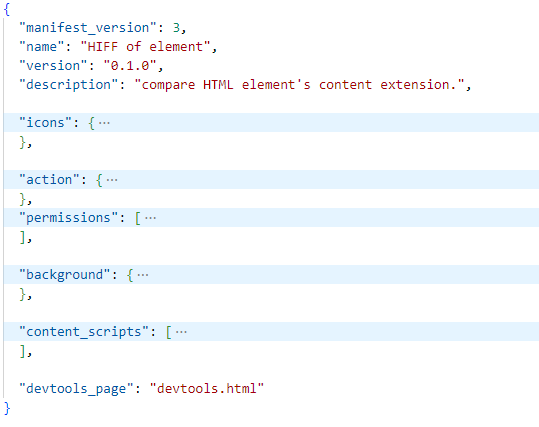
\includegraphics[width=0.6\textwidth]{picture/ch2-manifest.png}
    \caption{Manifest安裝檔範例}
    \label{f2.4}
\end{figure}

\subsection{內部腳本}\label{s2.6.3}
在擴充元件的架構中,根據不同的時機,也有不同的腳本來專門處理同類型的事件,以下列出常用腳本所負責的功能:
\begin{itemize}
    \item[●] Background Script: 一個擴充元件中,專門在背景頁面中執行的腳本,通常是處理程式中的主要邏輯。
    \item[●] Content Script: 作為Inspected window和擴充元件其他腳本溝通的管道,
    可以利用此腳本操控指定網頁下的元件或建立元件的監聽器,
    進而提供與網頁內容的相關功能。
    \item[●] Popup Script: 瀏覽器中右上角有個擴充元件的頁面按鈕,內部有個獨立的頁面,可以在裡面處理獨立的資訊和畫面。
    \item[●] DevTools Script: 在瀏覽器的Developer Tools中,可以建立子頁面來建立自訂義的功能或透過其他工具頁面來取得相關開發者訊息。
\end{itemize}

如圖\ref{f2.5}所示,一個擴充程式擁有一個background Page、多個content script和多個DevTools page的Panels...等等其他的頁面,
所有的擴充程式腳本除了Content script需要先指定好要與哪個Tab Id的Tab Content script溝通外,其餘的都可以自由的互相溝通。

不同的腳本中都有獨立的Scope,可以在內部存儲變數,但它們是不能直接存取對方的資料的,
例如:
Popup Script想要Background Script運算完的結果,
但他們無法互享溝通傳遞變數資料,只能透過Chrome中提供的通訊API,
利用Popup Script告訴Background Script想要你的資料,
Background Script才知道需要運算了並運算結束後結果回傳給Popup.js。

\indent
\begin{figure}[H]
    \centering
    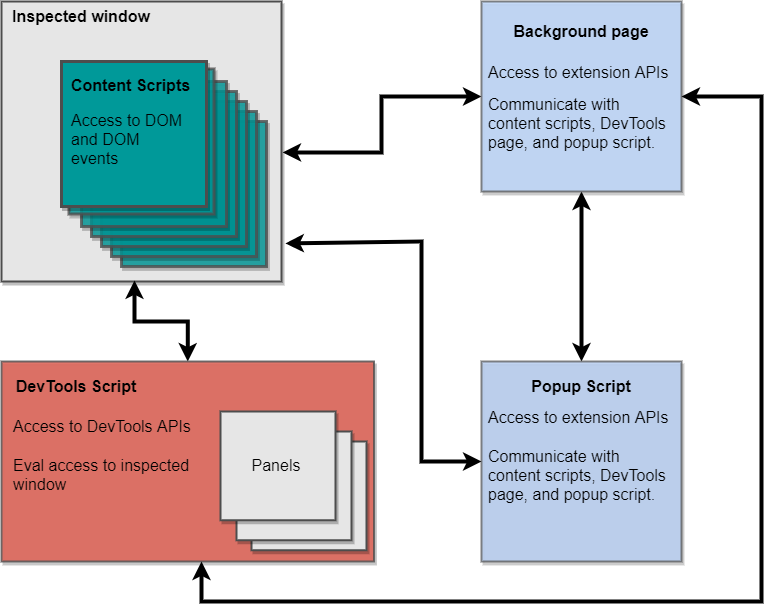
\includegraphics[width=0.9\textwidth]{picture/ch2-extension-script-relation.png}
    \caption{擴充程式腳本之關係圖}
    \label{f2.5}
\end{figure}
\chapter{Chrome擴充套件設計與實作}
\indent
在撰寫網頁測試腳本時,
為了避免網頁改版後,腳本內部中專門定位內部元件的Xpath無法正確抓取元件位置導致腳本頻頻出錯,
需要提高專門定位網頁中元件Xpath表達式的穩定性。

本論文以呂昭陞"提出提升穩定性的Xpath撰寫樣式"論文中的觀念為基礎,尋找符合的限制條件並建立一個穩定性高的網頁測試腳本,
但對於需要找出好的限制條件,對測試人員會是需要一定的經驗且較花時間的事情。
因此本論文提出在測試人員需要找尋適合的條件的時候可以透過Chrome擴充套件增加比較HTML文檔和過濾自訂屬性...等等額外功能的設計,
讓使用者即使在大型架構的HTML中也可以減少對於測試人員屬於雜訊的元件,可以較快速的挑選出想要屬性來設定適合的條件,
來撰寫適合定位該元件的Xpath表達式。

% =========================================================================================
% =========================================================================================
\section{擴充元件之使用情境}\label{s3.1}

在章節\ref{s2.4}有提到Xpath的組成方式,分別是Axis、Node test和零個或多個Predicate。
為了確保表達式中的穩定性,通常在設計時,都會同時使用這三種原件來組成一個路徑表達式。

在撰寫測試腳本時,每做完一個元件互動後,通常都需要驗證有相互關係的元件有出現或消失以確保該元件互動有確實被執行,
這時可以利用元件屬性的變化或元件的增減來當Xpath的限制條件,若畫面沒有執行該變化,代表利用此Xpath無法定位該元件,程式會將會執行失敗。
換句話說,若使用者要用一段Xpath表達式來判斷他是否有互動成功,必須要先找出它有哪些變化並加入在Xpath的條件中,
以圖\ref{f3.1}舉例,點擊了按鈕後,
HTML文本中會發現div元件中的class會從"status-one"變成"status-two",
若要用一段xpath表達式來確保有點擊按鈕,
可以撰寫成\colorbox{lightgray}{//div[@class="status-two"]//p[text()="Status msg"]},
如果網頁有問題,互動後元件中的class屬性沒有改變的話,上述Xpath中\colorbox{lightgray}{@class="status-two"}的條件會無法符合,
即無法定位到該元件位置,導致測試腳本執行失敗。

\begin{figure}[H]
    \centering
    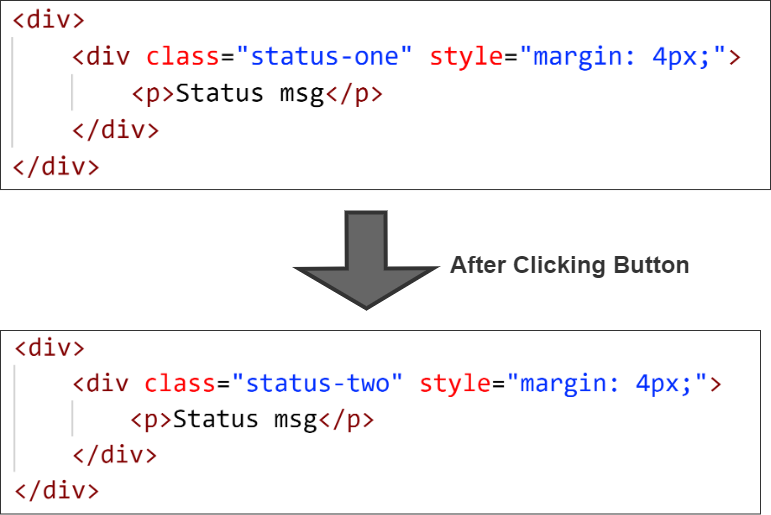
\includegraphics[width=0.6\textwidth]{picture/ch3-html-after-change.png}
    \caption{互動後HTML文本改變之範例圖}
    \label{f3.1}
\end{figure}

由上述例子可知,HTML變化後的元件或屬性很適合在測試腳本中當作互動是否成功的判斷。
一般使用者需要查看當下網頁中HTML會打開瀏覽器中的Developer Tools,
藉由Developer Tools中"Inspect Element"的功能,直接跳轉到點選物件的位置來查看元件的變化。
使用者在尋找元件變化的時候,常常會遇到以下兩種變化:

\begin{itemize}
    \item\textbf{元件互動時HTML文本快速變化}

    使用者在網頁中元件有互動行為的時候,
    可以在Developer Tools中觀察HTML文本因為互動而使元件內容或屬性產生快速的變化,
    如圖\ref{f3.2}所示,變化的元件會有紫色的漸淡背景框來提醒使用者。
    通常在元件屬性比較冗長複雜的情況下,
    元件的快速變化會造成使用者可能無法立即觀察出變化,
    需要花較多的時間重複元件互動行為來判斷它其中的差異。

    \begin{figure}[H]
        \centering
        \includegraphics[width=1.0\textwidth]{picture/ch3-element-change-fast.png}
        \caption{HTML互動後元件變化之顯示}
        \label{f3.2}
    \end{figure}
    
    \item\textbf{HTML文本未展開無變化提示}

    通常使用者會利用Developer Tools中"Inspect Element"的功能來找出元件在HTML中的位置,
    在使用這個功能時,會自動展開該元件上層的所有直屬元件,
    因為它只會幫你展開直屬元件,
    若未展開的元件或在Developer Tool中Element頁面需要滾動才看的元件有變化的話,
    較容易會被使用者忽略,
    以圖\ref{f3.3}為例,
    左半部的圖是未展開的狀態,在未展開時,紅色框內的元件並沒有紫色的漸淡背景框,
    若和右半部的圖一樣把元件展開後,才能發現裡面元件的變化並有紫色的漸淡背景框來提示使用者。

    \begin{figure}[H]
        \centering
        \includegraphics[width=1.0\textwidth]{picture/ch3-element-change-nghide.png}
        \caption{HTML文本未展開導致不會顯示變化提示}
        \label{f3.3}
    \end{figure}
    
\end{itemize}

因為上述兩種原因,會導致找出變化會花較多時間,
在此情況下可以使用此工具利用文本比較的方式把HTML中相異的地方列出,
讓測試人員可以使用工具所列出的差異來設計Xpath,來避免忽略掉較難找出的變化。

% =========================================================================================
% =========================================================================================
\section{系統架構}\label{s3.2}
圖\ref{f3.4}為Chrome擴充套件實作的系統架構圖,下列為各元件之介紹:

\begin{itemize}
\item\textbf{Chrome:}
以市占率第一的Chrome瀏覽器為背景下,對瀏覽器擴充元件進行實作

\item\textbf{Chrome Extension:}
對Chrome瀏覽器加裝此擴充功能之擴充程式

\item\textbf{Background Script For Extension:}
擴充程腳本之一, 屬於擴充元件的背景程序,通常會將程式的主要邏輯放在此腳本中

\item\textbf{SidePanel Script For Extension:}
擴充程式腳本之一, 在擴充元件Element頁面下的子頁面

\item\textbf{HTML Compare Function:}
比對兩個HTML差異之程式模組

\item\textbf{UI Interface:}
擴充元件在SidePanel裡面的使用者介面設計

\item\textbf{Test Script:}
針對Compare Function的單位測試腳本

\end{itemize}

\begin{figure}[H]
    \centering
    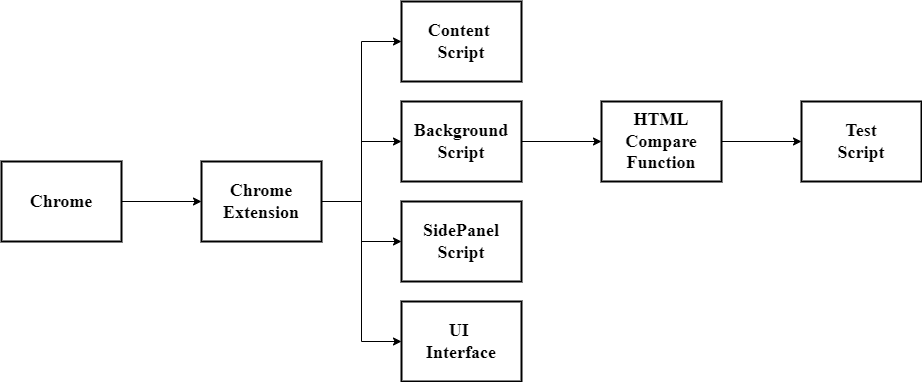
\includegraphics[width=0.9\textwidth]{picture/ch3-systemStucture.png}
    \caption{擴充元件實作之架構圖}
    \label{f3.4}
\end{figure}

此設計架構主要是以HTML比對函數為主,利用Chrome Extension的專用腳本們,把網頁的HTML讀取後丟入該比對系統,
比對完再進行回傳動作,最後利用UI介面把結果顯示在畫面上。

% =========================================================================================
% =========================================================================================
\section{HTML比對之實作}\label{s3.3}
若確定要開始進行比對網頁中的HTML文本後,需要先取出先前和之後的兩個HTML文本,然後進行文本前後比對\cite{HTML-Comparison-Algorithm}。
此比對功能,使用了開源程式Hiff的架構,經過權重部分修改、輸出元件的調整以及增加相關測試腳本,
調整成適合擴充程式的內部核心程式,並將此實作放入擴充程式的Background Script中。圖\ref{f3.5}為HTML比對之活動圖。

\begin{figure}[H]
    \centering
    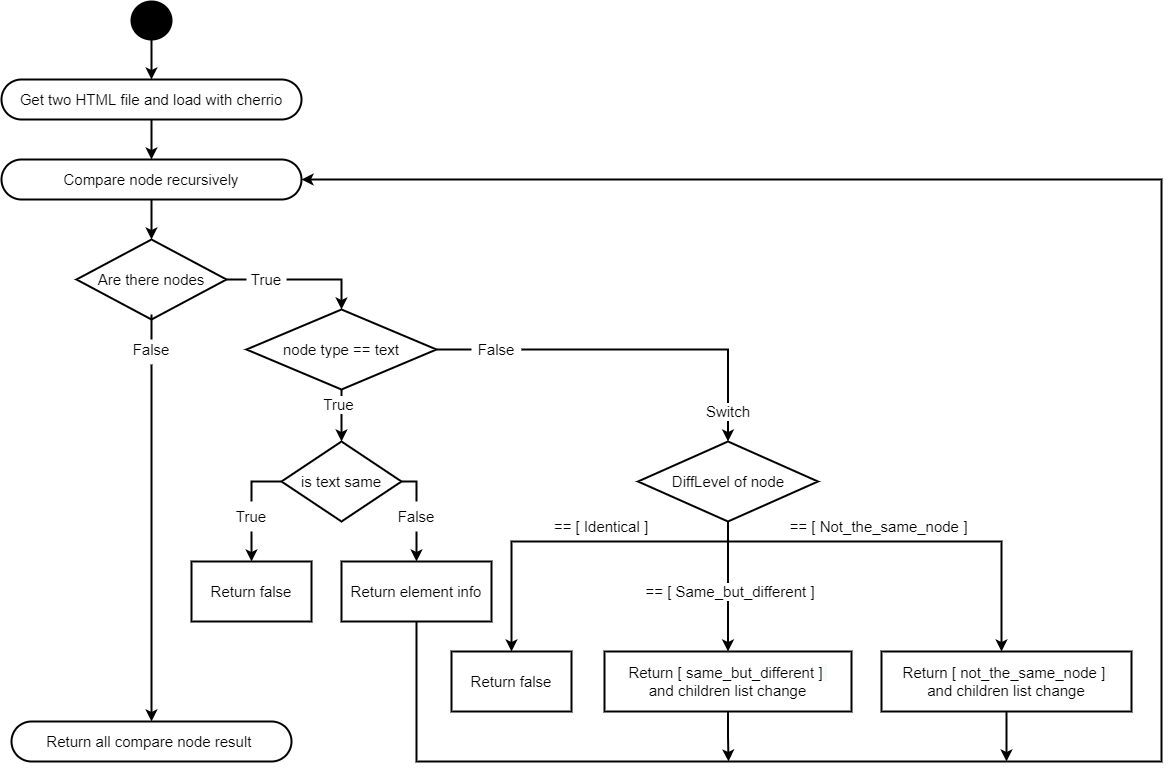
\includegraphics[width=1.0\textwidth]{picture/ch3-activity diagram.png}
    \caption{HTML比對之活動圖}
    \label{f3.5}
\end{figure}

\subsection{判斷節點相異程度}\label{s3.3.1}
在兩節點相互比對後,需要有一個判斷方法來確定該節點的相異程度,會分成三個等級:Identical、Same but different和Not the same node。
本程式的實作流程為圖\ref{f3.6},會先做比各屬性的比對,然後根據當前狀況選擇要該屬性自定義的權重,最後將所有權重相加來節點判斷相異等級

\begin{figure}[H]
    \centering
    \includegraphics[width=1.0\textwidth]{picture/ch3-HEURISTIC-comapre.png}
    \caption{節點相異程度之活動圖}
    \label{f3.6}
\end{figure}

\subsection{比對輸出結果}\label{s3.3.2}
在比對的時候有分成三種類型:Changed、Added和Removed,三種類型需要回傳相對應的資訊,
舊有的開源程式碼僅只有對該變更資訊用最低限度的字串來表示變更,經過修改後,將輸出結果加上變更節點的解析結果以及詳細屬性變化資訊,
在顯示上可以將結果直接輸出在畫面上,減少其他額外的處理。

在程式碼\ref{l3.1}為changed類型的輸出結果,
其中除了回傳相關的解析後的節點資訊,
裡面"info-compare"的值為比對該變化元件的所有類別結果,包括比對前、比對後和差異結果。

\begin{lstlisting}[caption=比對輸出結果(changed類型), label={l3.1}]
    1   function changed($nodeBefore, $nodeAfter) 
    2   {
    3    var before = grabParentAndIndex($nodeBefore),
    4    after = grabParentAndIndex($nodeAfter);
    5
    6    return {
    7    type: "changed",
    8    before:locationInfo(before.$parent, $nodeBefore, before.index),
    9    after: locationInfo(after.$parent, $nodeAfter, after.index),
    10   selectingNode: $nodeAfter,
    11   nodeINFO: $nodeBefore,
    12   info-compare: info_compare ($nodeBefore, $nodeAfter)
    13   };
    14  }
\end{lstlisting}

在程式碼\ref{l3.2}和程式碼\ref{l3.3}為added和changed類型的輸出結果,
其中除了回傳相關的解析後的節點資訊,
裡面"contentHTML"的值為added或removed元件的內部HTML資訊,會在UI介面中將整個變更的區塊告訴使用者。

\begin{lstlisting}[caption=比對輸出結果(added類型), label={l3.2}]
    1   function added($addedNode, $parentBefore, indexBefore, 
    2       $parentAfter, indexAfter) 
    3   {
    4     return {
    5     type: "added",
    6     before: locationInfo($parentBefore, undefined, indexBefore),
    7     after:  locationInfo($parentAfter, $addedNode, indexAfter),
    8     selectingNode: $parentAfter,
    9     nodeINFO: $addedNode,
    10    contentHTML: stringify($addedNode, false),
    11    };
    12  }
\end{lstlisting}

\begin{lstlisting}[caption=比對輸出結果(removed類型), label={l3.3}]
    1   function removed($removedNode, $parentBefore, indexBefore, 
    2       $parentAfter, indexAfter) 
    3   {
    4    return {
    5    type: "removed",
    6    before: locationInfo($parentBefore, $removedNode, indexBefore),
    7    after:  locationInfo($parentAfter, undefined, indexAfter),
    8    selectingNode: $parentAfter,
    9    nodeINFO: $removedNode,
    10   contentHTML: stringify($removedNode, false),
    11   };
    12  }
\end{lstlisting}


% =========================================================================================
% =========================================================================================
\section{擴充元件腳本設計之實作}\label{s3.4}
\indent
在章節\ref{s2.6.3}有對不同類型的腳本做基本介紹,針對各腳本獨特的特性分配它需要執行的功能。
圖\ref{f3.7}中表示出執行功能後的執行順序及流程,從按下比對文本的按鈕到比對結束的內部腳本們的流程圖。

\indent

\begin{figure}[H]
    \centering
    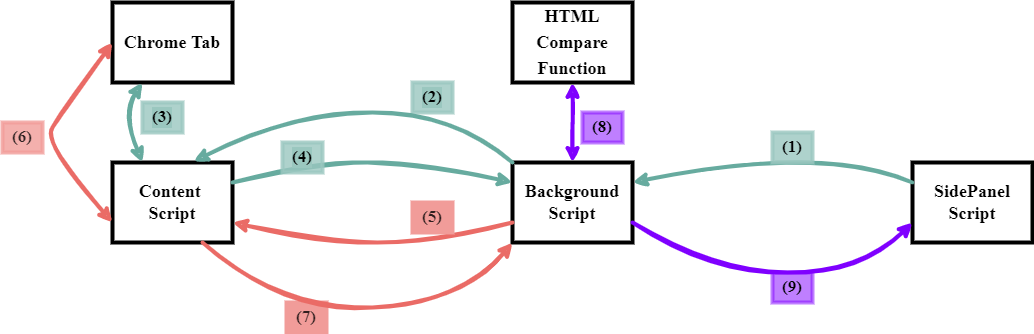
\includegraphics[width=1\textwidth]{picture/ch3-script-structure.png}
    \caption{擴充腳本之溝通順序圖}
    \label{f3.7}
\end{figure}

\subsection{SidePanel Script}\label{s3.4.1}
SidePanel Script是專門控制在Chrome Developer tools中Elements頁面中旁邊子介面的腳本,
此腳本主要功能在於若使用者點擊畫面中的互動按鈕或輸入相關字元,會讓擴充元件開始做動。
在UI介面下點擊開始比對的按鈕後,
等待第一個計時器結束後從Develope Tool中Elements頁面取出當下的HTML文本,
等待第二個計時器結束後再從Develope Tool中Elements頁面取出當下的HTML文本,
共取出變更前以及變更後的兩個HTML文本。
得到兩個文本後,便開始與Background Script溝通讓它知道要開始要進行比對了,
等到比對完後從Background Script得到結果並且把結果回傳給SidePanel Script,
最後將結果顯示在UI介面上,
如圖\ref{f3.7}中的(1)、(2)、(3)、(4)所示。

\subsection{Background Script}\label{s3.4.2}
Background Script在擴充元件中的定位是在背景中執行的程式,開發者通常將此程式的主要邏輯撰寫在這腳本中,
而HTML比對腳本的函數也是在此腳本中執行的,
接收到從SidePanel Script傳來的兩個HTML文本後便會開始比對,
比對後會將最後的比對結果回傳到SidePanel Script中,
如圖\ref{f3.7}中的(5)、(6)、(7)所示。


\section{UI/UX介面之實作}\label{s3.5}
設計此工具,為考慮人性化的使用介面以及比對後的結果方便使用者挑選所需要的條件,將此工具分成以下五個部分:
\begin{itemize}
    \item\textbf{Illustrate:}
    
    說明此擴充工具功能並且敘述該工具選擇的設定方式以及使用流程。

    \item\textbf{Timer:}
    
    依照使用者當前的網路狀況、元件互動情況...等等因素,藉由調整以下兩個Timer來調整抓取HTML文本的時間,

    \begin{itemize}
        \item\textbf{Time Of Set Up}
        
        在點擊"Start Compare"後,此Timer開始倒數計時,等到時間到後,便會抓取第一次的HTML文本。
        此Timer設計是為了讓使用者自定義一個充足的時間設定開始的狀態,讓使用者可以保持一個可控制的環境。
        例如:使用者想要抓取元件原本是Hover狀態到沒有Hover狀態的變化過程,
        可以設定此Timer,讓使用者可以在點擊按鈕後有充足的時間將滑鼠Hover到該元件上。

        \item\textbf{Time Of Change Element}
        
        等"Time Of Set Up"的時間結束並抓取第一次的HTML文本後,
        此Timer開始倒數計時,等到時間到後,
        便會將兩次的HTML文本一同傳送給Background Script執行比對。
 
    \end{itemize}
    
    \item\textbf{Options:}
    
    針對當前使用者狀態,透過選擇對應狀況的選項,讓使用者可以過濾掉大多數不需要的結果

    \begin{itemize}
        \item\textbf{Ignore style attribute's change}
 
        在HTML文件樣式中,有時會利用<style>標籤來建立簡易的CSS指令,但通常在使用時,較少用此標籤來設定條件,
        為避免有很多節點因為style屬性變化,造成比對結果較多不必要的資訊,故設立此條件來篩選。

        \item\textbf{Only display change of current selecting elemnt}
        
        若當前的HTML文本結構過大,但使用者僅僅只是要查看當前節點的變化,過多的變更結果會讓使用者較難找到適合當下情況的條件,
        為過濾掉當前節點之外的變更雜訊,在Develope Tool中Element頁面點擊HTML的節點,比較後的顯示結果僅會出現該節點的變化結果。
        
        \item\textbf{Display one tag's change}
        
        為避免比較後的結果過多,故添加了過濾元件tag的選項,
        讓使用者可以利用節點的tag過濾比對後的結果,例如:div、button...等等類別。

    \end{itemize}
    
    \item\textbf{Compare Control:}
 
    內部有兩個按鈕以及顯示比較情況的顯示框,可以點擊按鈕開始比對或點擊按鈕強制停止比對
    
    \item\textbf{Compare Result:}

    此面板中的下拉選單有顯示三中累行的結果:changed-area、added-area和removed-area,點擊後會出現表格顯示該節點的屬性比對,
    內部表格顯示該節點所有屬性的before、after和diff比對結果
    
    \end{itemize}
\indent

\begin{figure}[H]
    \centering
    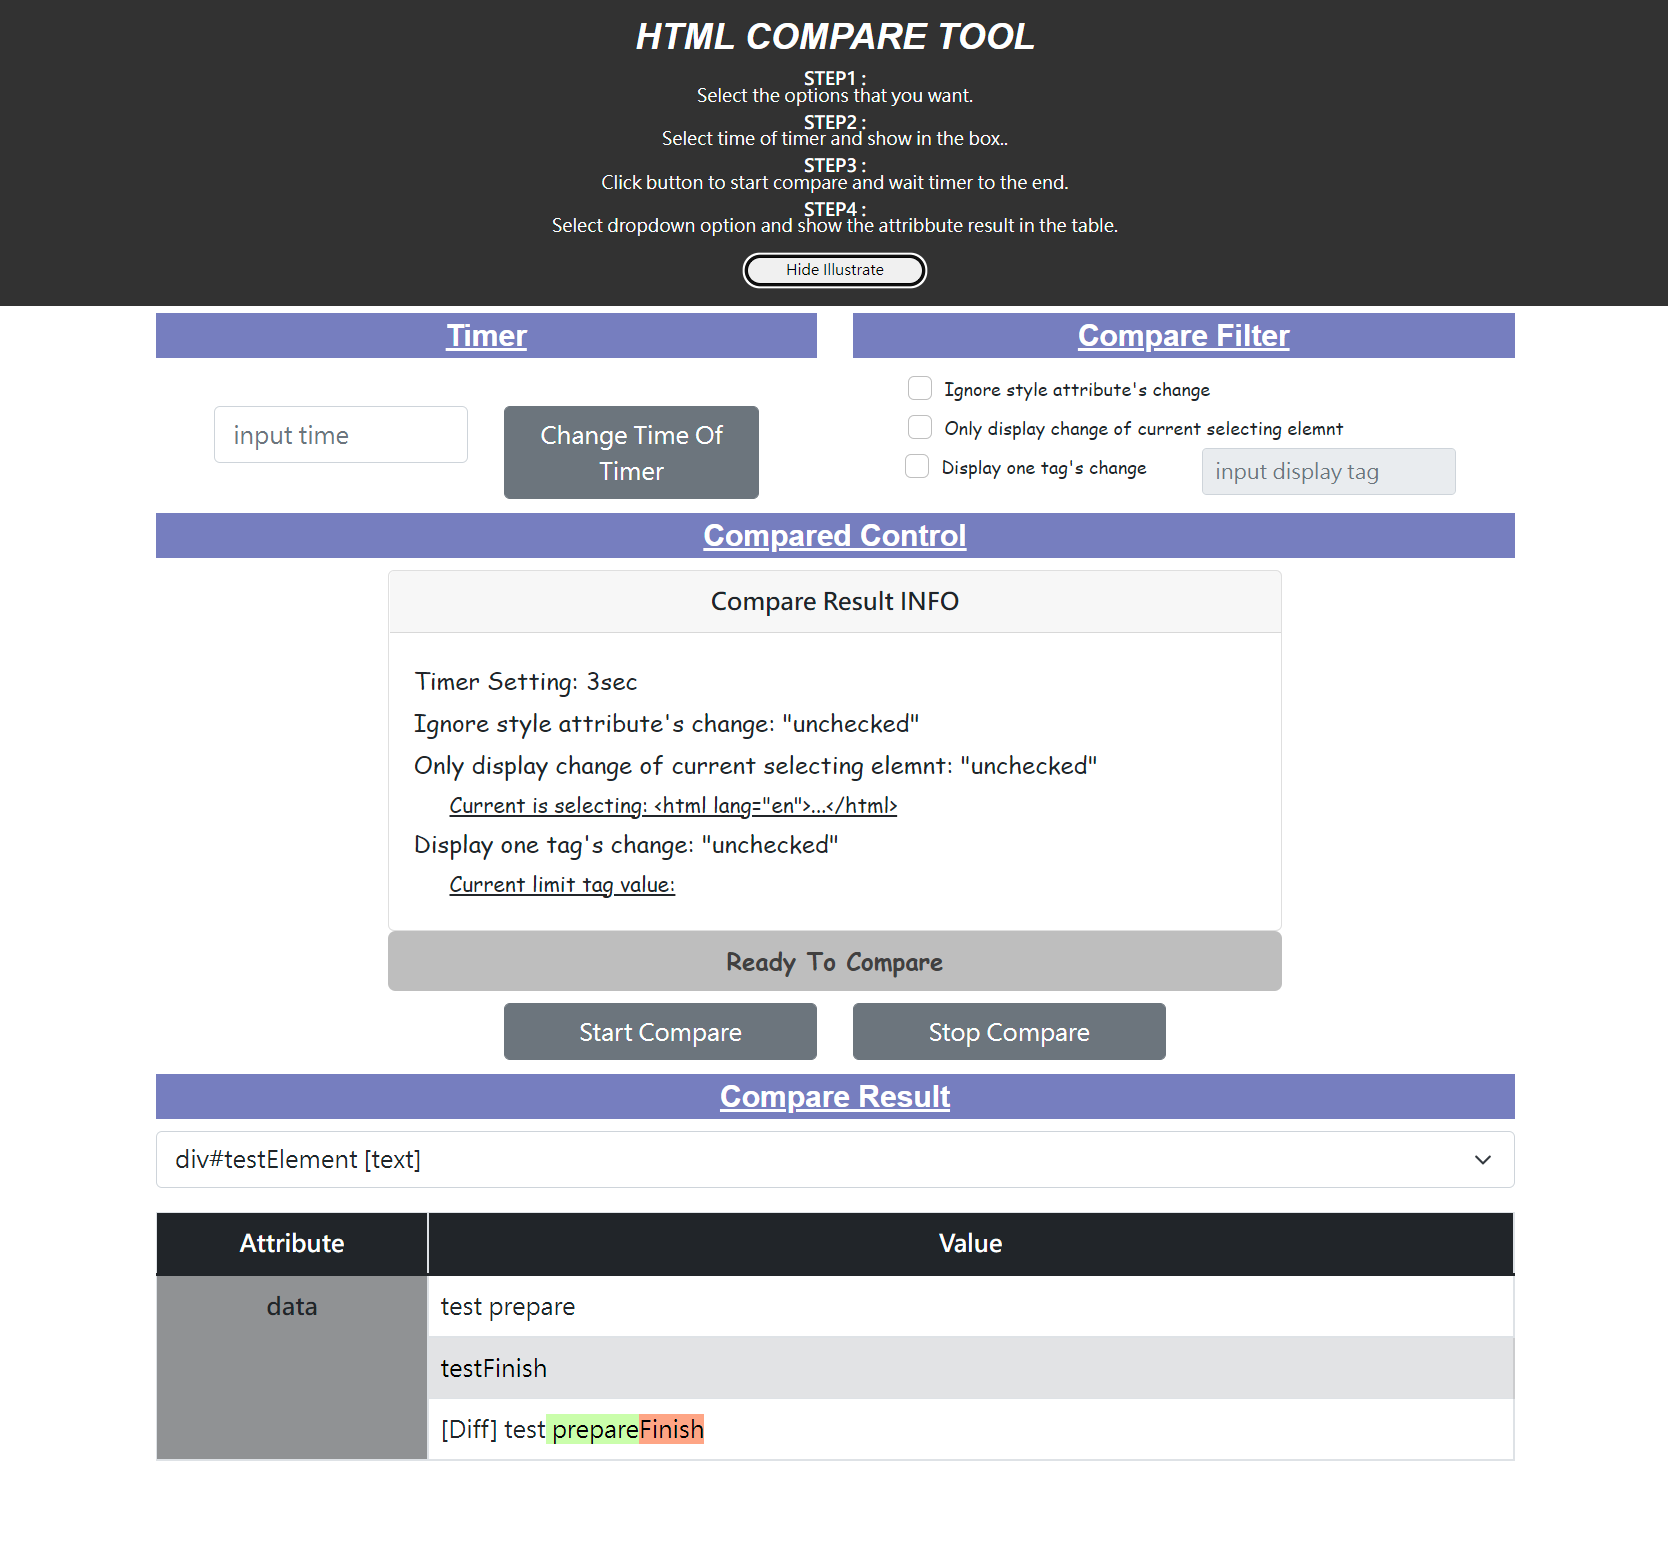
\includegraphics[width=1\textwidth]{picture/ch3-UIUX-example.png}
    \caption{UI設計之介面}
    \label{f3.8}
\end{figure}
\chapter{案例分析}
\section{案例實驗設計}\label{s4.1}
\indent
本論文提出的工具適用於畫面出現變化的情況,因此在實驗網站的挑選上,會以互動功能較多的網站為第一優先。
在眾多的模板網頁中,圖\ref{f4.1}所示的家具銷售模板網站\cite{Furn-Free-CSS-Template}符合互動多的特性,
因此本實驗的實驗網站以該網站為基礎來做修改。
本論文的實驗案例是基於撰寫測試腳本時常會遇到的情況下,
挑選出五個情境並設計成符合實驗網頁的情境來讓實驗人員實際操作。

\begin{figure}[H]
    \centering
    \setlength{\abovecaptionskip}{-5pt}
    \setlength{\belowcaptionskip}{0pt}
    \includegraphics[width=0.88\textwidth]{picture/experiment/test-environment-demo.png}
    \caption{實驗模板網站}
    \label{f4.1}
\end{figure}

在實驗人員的選擇的部分,
將以有資工相關背景為優先選擇並邀請到14位皆為臺北科技大學資工系的學生,
其中包含大二、大三的專題生和碩士一年級、二年級的同學,
並將它們分成七位有網頁測試相關經驗和七位對此技術較為陌生兩種類別的人。
為因應目前疫情時間,測試環境皆在同一台電腦進行操作,
實體操作則直接操作電腦,
遠端操作則使用Window遠端連線到該電腦來進行操作。
另外,為確保實體和遠端的操作環境相同,遠端設備皆會檢測網速在至少在100Mbps以上,並確保操作畫面時不會有遲鈍的現象。
操作的鍵盤滑鼠均使用實驗者平時在使用的設備,
實驗人員的操作介面為Chrome瀏覽器,工具為Chrome瀏覽器中的Developer Tools和本實驗提出的擴充元件。
在實驗過程中,會確保實驗人員在只有一個人的環境中進行案例實作以及排除任何會影響實驗準確性之外在因素,
例如:手機、通訊軟體、開啟其他瀏覽器分頁等等

實驗流程開始前,
會先對實驗人員用同一個簡報簡易說明該論文的背景知識、測試目的以及實驗網頁的簡單介紹,
之後會示範操作一個簡易的範例並且讓實驗人員親自操作此範例來熟悉該工具,
一切初始程序就位後才會開始操作實驗案例。
操作實驗案例的流程為先講解實作案例的情境,確認實驗人員了解後開始計時,直到實驗人員找出結果後才停止計時,
每位實驗人員皆會操作實驗章節\ref{s4.2}提到的五個實驗案例,
先以只使用Developer Tools的情況下實作五個實驗案例,
再以使用Developer Tools加上擴充元件的情況實作五個相同實驗案例。
等待14位實驗人員操作完成後,統整所有實驗人員的相關數據並以是否有使用本實驗提出擴充元件和是否有相關經驗兩種因素進行實作時間比較,

\section{測試案例實作}\label{s4.2}

\subsection{案例一:Hover購物車圖示後出現購物車下拉式畫面}\label{s4.2.1}
\indent
實驗人員的測試情境為將滑鼠放在購物車的圖示上,
等到下拉式畫面出現後,需要找出所有因為下拉式畫面出現而屬性變化的元件,如圖\ref{f4.2}所示。

該案例共有兩個元件產生屬性變化,如果實驗人員皆找出變化並指出在Dev Tools中的位置則計為成功並記錄秒數。

\begin{figure}[H]
    \centering
    \setlength{\abovecaptionskip}{-5pt}
    \setlength{\belowcaptionskip}{0pt}
    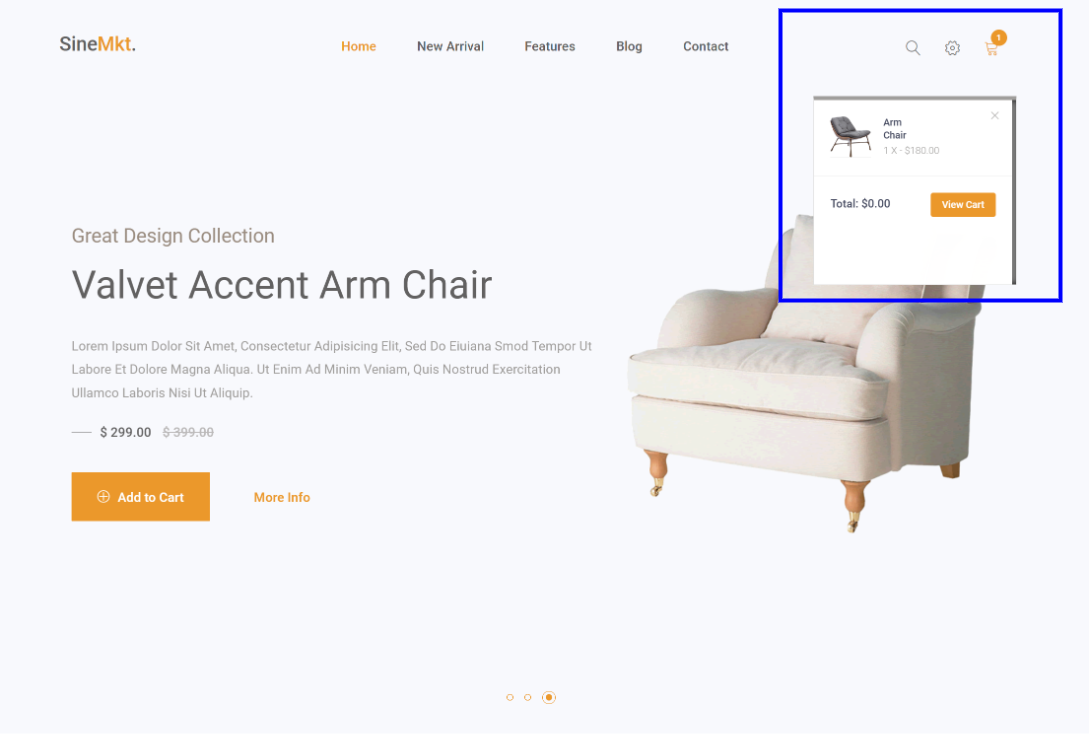
\includegraphics[width=0.9\textwidth]{picture/experiment/test-environment-no1.png}
    \caption{Hover購物車圖示後出現下拉示畫面之網頁變化}
    \label{f4.2}
\end{figure}

\subsection{案例二:點擊搜尋框後,僅需要了解該元件屬性變化}\label{s4.2.2}
\indent
實驗人員的測試情境為點擊搜尋圖標後,將隱藏的搜尋框展開,
並找出有因為此互動而有變化的元件,如圖\ref{f4.3}所示。
該案例需要找出一個指定元件的屬性變化,如果實驗人員皆找出變化並指出在Dev Tools中的位置則計為成功並記錄秒數。
在此情境中,實驗人員可以使用擴充元件中``Only display change of current selecting element''的Option,
讓實驗人員可以利用該Option過濾掉其餘畫面中不是搜尋框的變化,並指出在Dev Tools中的位置,讓實驗人員專注在指定元件的屬性中。

\begin{figure}[H]
    \centering
    \setlength{\abovecaptionskip}{-5pt}
    \setlength{\belowcaptionskip}{0pt}
    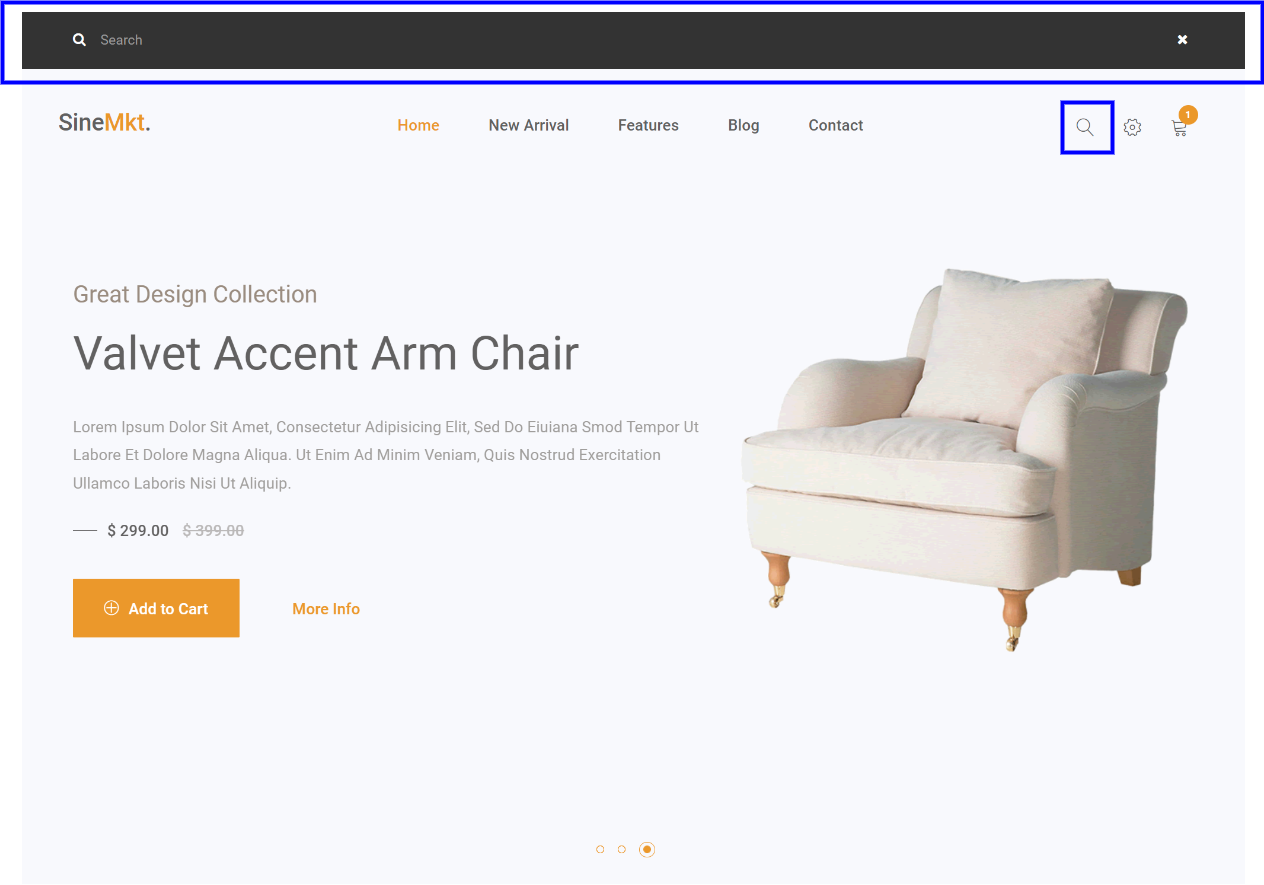
\includegraphics[width=0.9\textwidth]{picture/experiment/test-environment-no2.png}
    \caption{點擊搜尋圖標後之網頁變化}
    \label{f4.3}
\end{figure}

\subsection{案例三:網頁中畫面定時更換內容}\label{s4.2.3}
\indent
實驗人員的測試情境為在網頁中的產品促銷頁面更換的情況下,
找出因為畫面更換而屬性出現變化的元件。
在此產品促銷頁面中,有三個子頁面,裡面各有一個促銷商品。
若實驗人員的滑鼠鼠標沒有在促銷頁面上,
它會定時切換至不同的頁面中,
實驗人員可以在不用操作頁面的情況下,
看到每個在頁面上的促銷商品,
也可以點擊下方的小圓點手動切換畫面,
如圖\ref{f4.4}所示。

該案例需要找出四個元件的屬性變化,如果實驗人員皆找出變化並指出在Dev Tools中的位置則計為成功並記錄秒數。

\begin{figure}[H]
    \centering
    \setlength{\abovecaptionskip}{-5pt}
    \setlength{\belowcaptionskip}{0pt}
    \includegraphics[width=0.9\textwidth]{picture/experiment/test-environment-no3.png}
    \caption{產品促銷頁面循環示意圖}
    \label{f4.4}
\end{figure}


\subsection{案例四:點擊上方導覽列跳轉到該類別畫面}\label{s4.2.4}
\indent
實驗人員的測試情境為點擊網頁上方的導覽列,
可以快速跳轉到該網頁的指定區塊,
讓實驗人員不用花費多餘的時間尋找該區塊在頁面中的位置,如圖\ref{f4.5}所示。
一般在畫面快速跳轉的情況下,
無法快速地知道那些元件屬性有改變到,
且必須要從整個網頁中慢慢尋找,
透過此工具,
可以快速地呈現差異結果提供給實驗人員判斷是否適合當XPath表達式的條件。
該案例需要找出四個元件的屬性變化,
如果實驗人員皆找出變化並指出在Dev Tools中的位置則計為成功並記錄秒數。

\begin{figure}[H]
    \centering
    \setlength{\abovecaptionskip}{-5pt}
    \setlength{\belowcaptionskip}{0pt}
    \includegraphics[width=0.6\textwidth]{picture/experiment/test-environment-no4.png}
    \caption{利用導覽列跳轉到其他畫面之示意圖}
    \label{f4.5}
\end{figure}

\subsection{案例五:互動後當下網頁畫面無變化}\label{s4.2.5}
\indent
實驗人員的使用情境為點擊促銷頁面中的按鈕後,網頁下方標題``New Arrivals''下方會多一排文字。
正常狀況下,
在點擊按鈕時,標題``New Arrivals''是沒有在畫面中的,
導致實驗人員在點擊後看不到網站的變化。
因為產生變化的元件沒有在畫面中,
無法使用Developer Tools中``Inspect Element''的功能定位到該元件附近,
在未展開元件的情況下,也無法看見紫色漸淡背景框,
實驗人員只能上下滑動頁面觀察網頁畫面的變化來找出新增的元件,如圖\ref{f4.5}所示。
該案例需要找出一個被添加的元件,如果實驗人員找出變化並指出在Develope Tool中的位置則計為成功並記錄秒數。

\begin{figure}[H]
    \centering
    \setlength{\abovecaptionskip}{-5pt}
    \setlength{\belowcaptionskip}{0pt}
    \includegraphics[width=1.0\textwidth]{picture/experiment/test-environment-no5.png}
    \caption{當下網頁中無包括有變化的元件之示意圖}
    \label{f4.6}
\end{figure}

\newpage

\section{實驗數據分析}\label{s4.3}
\indent
本次實驗共有14位實驗人員參與,分成無相關經驗的7位以及有相關經驗的7位,藉由實驗人員的操作時間來比較有無使用此工具之差別。
表\ref{t4.1}、\ref{t4.2}使用的A符號,代表是無使用擴充程式的情況下;使用的B符號,代表是有使用擴充程式的情況下。

\subsection{無相關經驗實驗人員實例操作時間比較}\label{s4.3.1}
表\ref{t4.1}為紀錄無相關經驗的實驗人員在不同的實例下,分別使用兩種不同的尋找XPath路徑條件方法來比較其花費的時間,
從表中可見每一位實驗者大部分的實例是使用擴充工具會有明顯的改善,極少數會有使用擴充工具較慢的情況。
但從圖\ref{f4.7}可以明顯看出在五個案例的平均數據中,
使用擴充工具所花費的時間有明顯的降低,
減少的時間達25\%以上,案例五甚至有高達70\%左右。

\begin{table}[H]
    \begin{center}
    \setlength{\abovecaptionskip}{10pt}
    \setlength{\belowcaptionskip}{-10pt}
    \caption{無相關經驗的實驗人員在有無使用擴充工具的情況下比較五個實例操作時間}\label{t4.1}
        \begin{tabular}{|c|c|c|c|c|c|c|c|c|}   \hline
        & 人員1   & 人員2   & 人員3   & 人員4   & 人員5   & 人員6   & 人員7    & \textbf{平均時間}\\\hline\hline
        實例一 [A]   & 02m34s    & 02m14s    & 01m24s    & 02m58s    & 01m32s    & 02m07s    & 03m17s    & \textbf{02m18s}\\\hline
        實例一 [B]   & 02m10s    & 01m50s    & 01m15s    & 02m13s    & 00m38s    & 01m37s    & 02m03s    & \textbf{01m41s}\\\hline\hline
        實例二 [A]   & 04m38s    & 01m36s    & 00m41s    & 01m19s    & 01m12s    & 02m38s    & 01m22s    & \textbf{01m55s}\\\hline
        實例二 [B]   & 01m03s    & 00m54s    & 00m56s    & 01m05s    & 00m53s    & 01m07s    & 00m58s    & \textbf{00m59s}\\\hline\hline
        實例三 [A]   & 03m06s    & 03m36s    & 03m09s    & 04m38s    & 00m53s    & 03m30s    & 03m26s    & \textbf{03m11s}\\\hline
        實例三 [B]   & 01m21s    & 03m11s    & 01m23s    & 02m50s    & 01m15s    & 01m15s    & 02m36s    & \textbf{01m59s}\\\hline\hline
        實例四 [A]   & 03m28s    & 03m19s    & 02m45s    & 02m30s    & 02m47s    & 03m52s    & 04m03s    & \textbf{03m15s}\\\hline
        實例四 [B]   & 01m37s    & 02m11s    & 01m31s    & 02m57s    & 01m37s    & 02m51s    & 02m38s    & \textbf{02m12s}\\\hline\hline
        實例五 [A]   & 04m20s    & 02m51s    & 02m30s    & 04m16s    & 03m01s    & 01m43s    & 01m05s    & \textbf{02m49s}\\\hline
        實例五 [B]   & 01m26s    & 00m38s    & 00m32s    & 01m19s    & 00m30s    & 00m31s    & 00m35s    & \textbf{00m47s}\\\hline\hline
        \end{tabular}
    \end{center}
\end{table}

\begin{figure}[H]
    \centering
    \setlength{\abovecaptionskip}{-15pt}
    \setlength{\belowcaptionskip}{0pt}
    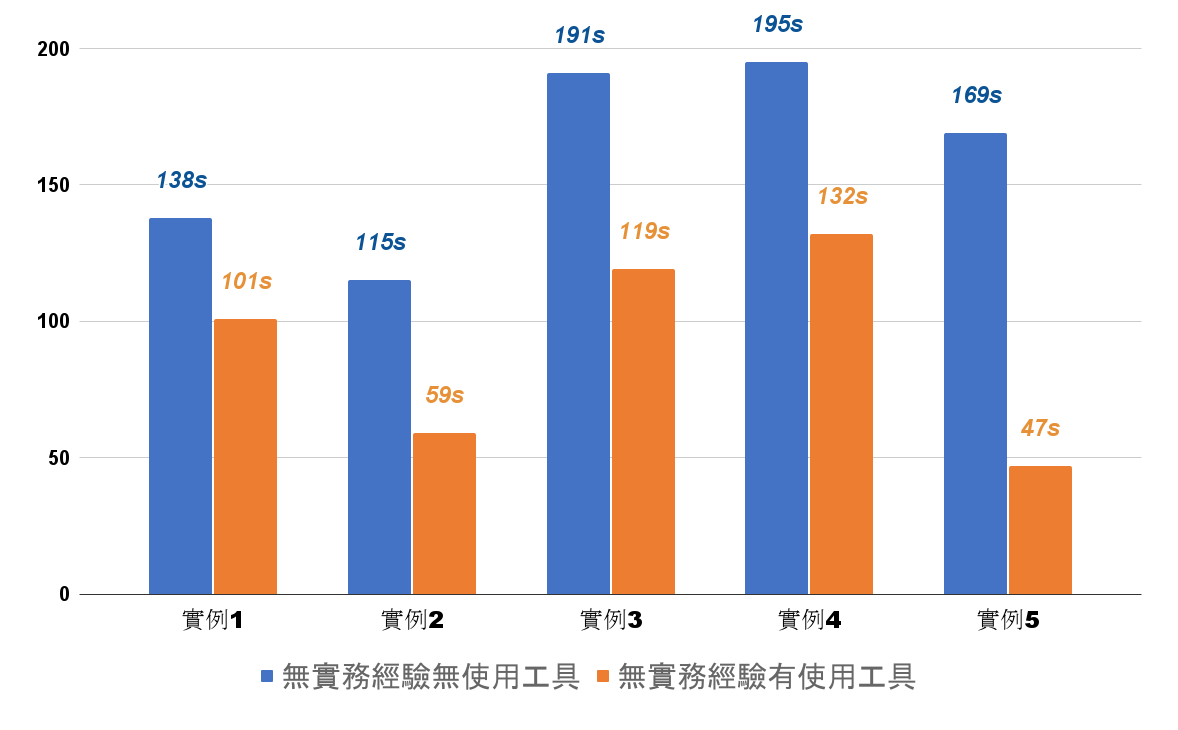
\includegraphics[width=0.87\textwidth]{picture/experiment/ch4-no_experience_compare.png}
    \caption{無相關經驗有無使用工具之比較(單位:秒)}
    \label{f4.7}
\end{figure}

\subsection{有相關經驗實驗人員實例操作時間比較}\label{s4.3.2}
表\ref{t4.2}為紀錄有相關經驗的實驗人員在各個實例下使用兩種不同尋找XPath的方法之比較其花費的時間,
從表中可以發現,相較於無相關經驗的實驗人員,有相關經驗的實驗人員有無使用擴充工具的時間差異不大,甚至有時候會略慢。
在實驗的過程中有發現,在使用工具時,雖然可以快速找到變化,但無法快速找到變化元件的HTML位置,在章節\ref{s5.2.2}會對此情況探討,
但從圖\ref{f4.8}可以發現,
案例二雖然平均時間相近,
但案例二的實作過程只要找尋一個元件的變化,
有相關經驗的實驗人員平時在找尋條件時也都只會看當下的元件,若當下的元件沒有複雜且快速的變化,使用工具對當下的情境是不會特別有幫助的,所以案例二的結果是可以預期的。
雖然使用工具依然可以減少約20\%的花費時間,但減少的時間不如無相關經驗的實驗人員明顯。

\begin{table}[H]
    \begin{center}
    \setlength{\abovecaptionskip}{10pt}
    \setlength{\belowcaptionskip}{-10pt}
    
    \caption{有相關經驗的實驗人員在有無使用擴充工具的情況下比較五個實例操作時間}\label{t4.2}
        \begin{tabular}{|c|c|c|c|c|c|c|c|c|}   \hline
        & 人員1   & 人員2   & 人員3   & 人員4   & 人員5   & 人員6   & 人員7    & \textbf{平均時間}\\\hline\hline
        實例一 [A]   & 01m16s    & 02m17s    & 02m28s    & 02m19s    & 02m04s    & 02m11s    & 02m41s    & \textbf{02m11s}\\\hline
        實例一 [B]   & 00m58s    & 01m43s    & 01m50s    & 01m56s    & 01m36s    & 02m01s    & 02m49s    & \textbf{01m50s}\\\hline\hline
        實例二 [A]   & 01m10s    & 01m53s    & 01m17s    & 01m16s    & 00m58s    & 00m44s    & 01m19s    & \textbf{01m14s}\\\hline
        實例二 [B]   & 00m51s    & 01m40s    & 01m25s    & 00m59s    & 00m46s    & 01m00s    & 01m22s    & \textbf{01m09s}\\\hline\hline
        實例三 [A]   & 03m28s    & 02m12s    & 02m00s    & 04m20s    & 01m50s    & 01m22s    & 03m26s    & \textbf{02m40s}\\\hline
        實例三 [B]   & 01m24s    & 03m20s    & 01m20s    & 01m38s    & 01m09s    & 01m24s    & 02m57s    & \textbf{01m53s}\\\hline\hline
        實例四 [A]   & 02m40s    & 02m44s    & 02m40s    & 01m56s    & 02m15s    & 01m53s    & 02m30s    & \textbf{02m23s}\\\hline
        實例四 [B]   & 01m20s    & 01m52s    & 01m33s    & 01m27s    & 01m40s    & 01m10s    & 02m31s    & \textbf{01m39s}\\\hline\hline
        實例五 [A]   & 04m48s    & 02m26s    & 04m41s    & 02m29s    & 01m58s    & 01m53s    & 01m20s    & \textbf{02m48s}\\\hline
        實例五 [B]   & 00m30s    & 01m07s    & 00m47s    & 00m32s    & 00m27s    & 00m39s    & 00m37s    & \textbf{00m40s}\\\hline\hline
        \end{tabular}
    \end{center}
\end{table}

\begin{figure}[H]
    \centering
    \setlength{\abovecaptionskip}{-15pt}
    \setlength{\belowcaptionskip}{0pt}
    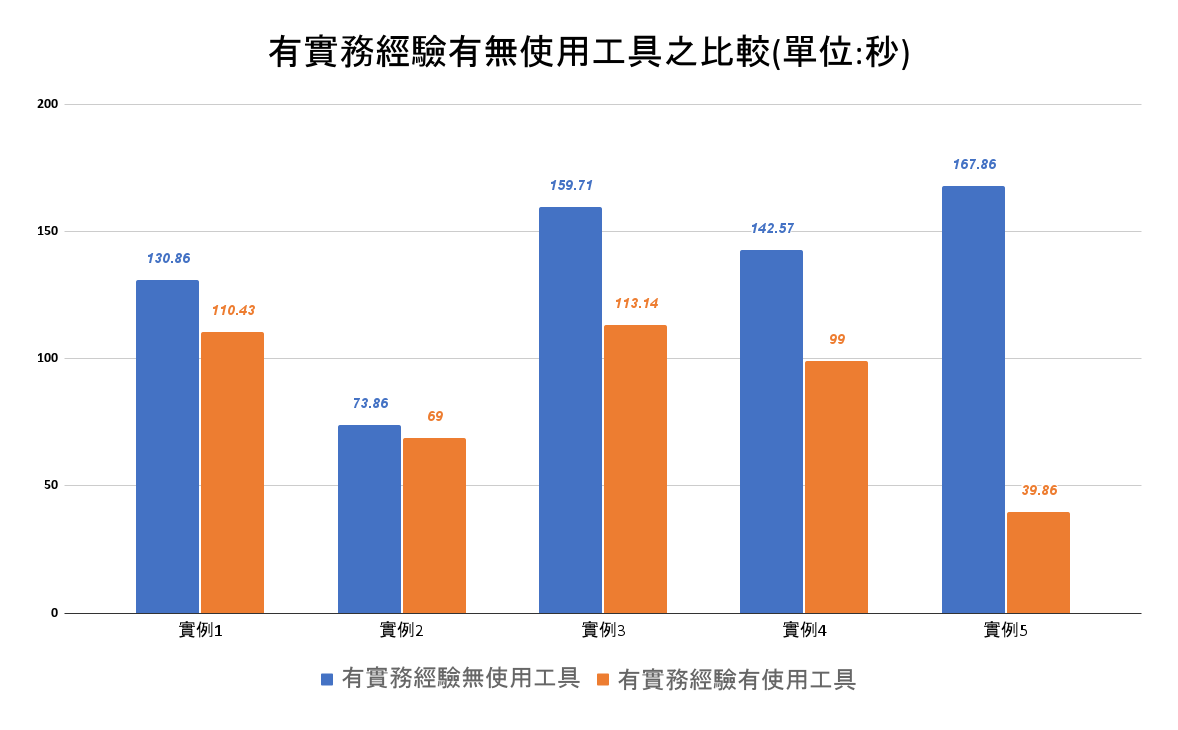
\includegraphics[width=0.87\textwidth]{picture/experiment/ch4-have_experience_compare.png}
    \caption{有相關經驗有無使用工具之比較(單位:秒)}
    \label{f4.8}
\end{figure}

\subsection{全體實驗人員實例操作時間比較}\label{s4.3.3}

由圖\ref{f4.9}的全部實驗人員平均時間統計結果,可以看出每個案例都減少$20\%\sim30\%$的時間,
其中案例五在有經驗或無經驗的情況下,使用擴充程式能使找尋變化的時間皆大幅減少,
由此可以看出即使有經驗的實驗人員,也較難找出超出畫面外的元件變化。

% \begin{table}[H]
%     \begin{center}
%     \setlength{\abovecaptionskip}{10pt}
%     \setlength{\belowcaptionskip}{15pt}
%     \caption{在無實務經驗情況下,是否使用擴充工具之五個實例操作時間比較}\label{t4.3}
%         \begin{tabular}{|c|c|c|c|}   \hline
%         & 無實務經驗人員平均   & 有實務經驗人員平均   & \textbf{總人員平均}\\\hline
%         實例一 [A]   & 02m18s   & 02m11s    & \textbf{02m14s}\\\hline
%         實例一 [B]   & 01m41s   & 01m50s    & \textbf{01m46s}\\\hline
%         實例二 [A]   & 01m55s   & 01m14s    & \textbf{01m35s}\\\hline
%         實例二 [B]   & 00m59s   & 01m09s    & \textbf{01m04s}\\\hline
%         實例三 [A]   & 03m11s   & 02m40s    & \textbf{02m55s}\\\hline
%         實例三 [B]   & 01m59s   & 01m53s    & \textbf{01m56s}\\\hline
%         實例四 [A]   & 03m15s   & 02m23s    & \textbf{02m49s}\\\hline
%         實例四 [B]   & 02m12s   & 01m39s    & \textbf{01m55s}\\\hline
%         實例五 [A]   & 02m49s   & 02m48s    & \textbf{02m49s}\\\hline
%         實例五 [B]   & 00m47s   & 00m40s    & \textbf{00m44s}\\\hline
%         \end{tabular}
%     \end{center}
% \end{table}

\begin{figure}[H]
    \centering
    \setlength{\abovecaptionskip}{-15pt}
    \setlength{\belowcaptionskip}{0pt}
    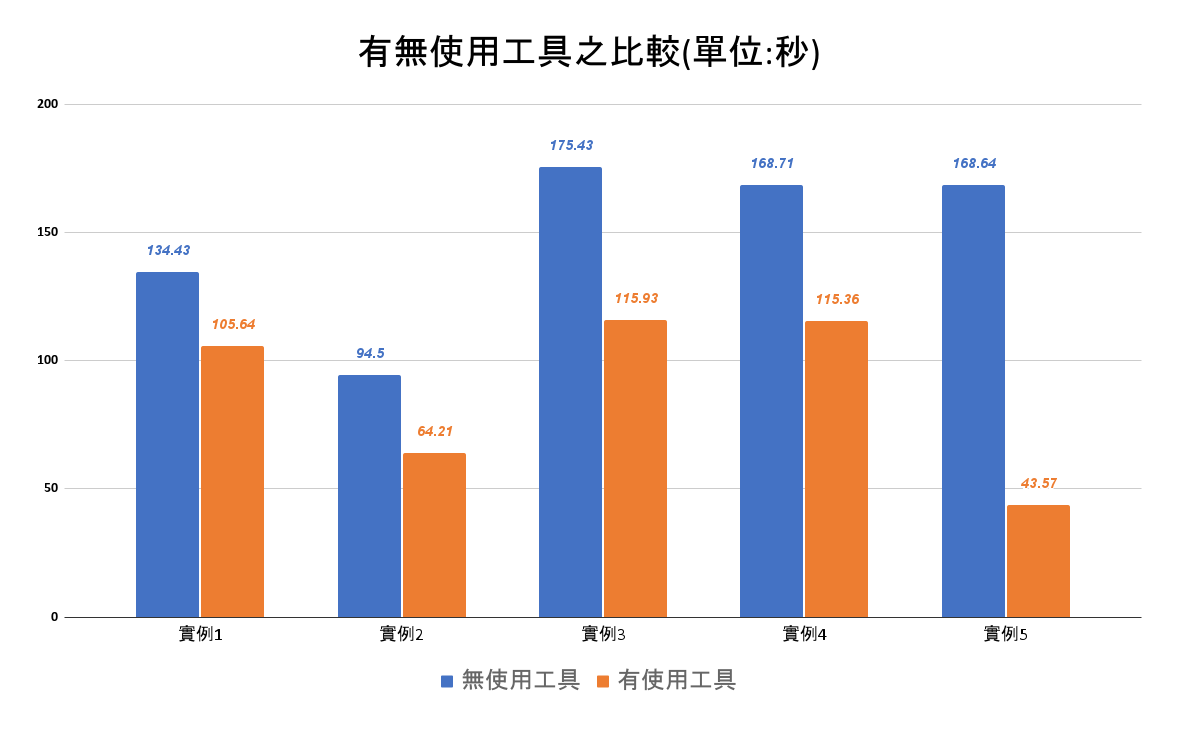
\includegraphics[width=0.87\textwidth]{picture/experiment/ch4-all_compare.png}
    \caption{有無使用工具之比較(單位:秒)}
    \label{f4.9}
\end{figure}


% \begin{table}[H]
%     \begin{center}
%     \setlength{\abovecaptionskip}{10pt}
%     \setlength{\belowcaptionskip}{20pt}
%     \caption{有相關經驗的情況下,是否使用擴充工具之五個實例操作時間比較}\label{t4.2}
%         \begin{tabular}{|c|c|c|c|c|c|c|c|}   \hline
%         & 人員1   & 人員2   & 人員3   & 人員4   & 人員5   & 人員6   & 人員7\\\hline
%         \makecell[l]{實例一 \\ (無使用擴充元件)}  & 06m02s    & 03m24s    & 04m20s    & 04m20s    & 04m20s    & 04m20s    & 04m20s    \\\hline
%         實例一 A  & 06m02s    & 03m24s    & 04m20s    & 04m20s    & 04m20s    & 04m20s    & 04m20s    \\\hline
%         1A  & 06m02s    & 03m24s    & 04m20s    & 04m20s    & 04m20s    & 04m20s    & 04m20s    \\\hline
%         1B  & 06m02s    & 03m24s    & 04m20s    & 04m20s    & 04m20s    & 04m20s    & 04m20s    \\\hline
%         \textbf{增減時間}    & \textbf{06m18s}    & \textbf{04m38s}    & \textbf{06m18s}    & \textbf{06m18s}    & \textbf{06m18s}    & \textbf{06m18s}    & \textbf{06m18s}    \\\hline
%         \textbf{增減比例}    & \textbf{06m18s}    & \textbf{04m38s}    & \textbf{06m18s}    & \textbf{06m18s}    & \textbf{06m18s}    & \textbf{06m18s}    & \textbf{06m18s}    \\\hline
%         \end{tabular}
%     \end{center}
% \end{table}
\chapter{結論與未來展望}
\section{結論}\label{s5.1}
\indent
本論文基於呂昭陞論文提出XPath撰寫樣式的使用前提下,
為減少在挑選適合的路徑條件所花用的時間,而提出利用HTML比對的瀏覽器擴充元件找出適合的元件定位條件。

使用者一般在查找變化時,通常都會使用瀏覽器中的Developer Tools來觀察元件是否有淺紫背景框,
但這個方法較慢又容易忽略一些更適合當成XPath路徑條件的變化。
此擴充元件透過HTML比對,將有變化的元件列舉出來,讓使用者可以直接透過結果挑選適合的變化加入XPath的路徑條件中。
從實驗結果可以得知,
無論是無相關經驗或已經有一定基礎的測試人員使用Developer Tools配合此擴充元件查找變化,
和僅使用Developer Tools的情況相比,時間減少$20\%\sim30\%$左右,
尤其無相關經驗的測試人員減少的時間會更多一些。
由此可知,透過Developer Tools加上擴充元件的輔助可以降低設計XPath所花用時間,提高撰寫測試腳本的效率。

\section{未來方向}\label{s5.2}
\indent
本論文提出之HTML比對工具仍有待改善之處,以下將分為五點說明:

\subsection{比較節點相異等級之演算法}\label{s5.2.1}

本論文使用的HTML比對程式,
計算節點相異的等級有分成``IDENTICAL''、``SAME BUT DIFFERENT''和``NOT THE SAME NODE''三種類型。
判斷節點相異的演算法是先設定每個屬性的權重,並將該節點所擁有的屬性權重全部相加,最後計算後的結果來決定該節點的相異等級。

使用這種演算法的時候,在判定``SAME BUT DIFFERENT''和``NOT THE SAME NODE''這兩種類型時,
沒辦法精確的判定相異等級,
像是圖\ref{f5.1}中以使用者的角度會知道它是id=``456''的節點刪除,
但以原本的演算法會因為節點等級,
而判斷成id=``456''的元件修改成id=``789''的元件,原本id=``789''的元件則會被刪除。
若能調整判斷節點的演算法,使它更能趨近使用者的結果,最後輸出的節點變化類型也會更精確。

\indent
\begin{figure}[H]
    \centering
    \includegraphics[width=0.8\textwidth]{picture/ch-5 Heuristic_improve.png}
    \caption{比較節點相異等級之情境}
    \label{f5.1}
\end{figure}

\subsection{比對相異之元件自動跳轉到Develope Tool中Element頁面並標記}\label{s5.2.2}

此工具在顯示結果時,僅告訴使用者變化元件的路徑,
使用者必須照著路徑一個一個慢慢找出元件在該HTML的位置,
或透過畫面上的元件變化直接用Developer Tools中``Inspect Element''功能找出元件後,再利用路徑查看是不是比較結果中的元件,
若以上述的兩種作法操作,使用速度及方便度會降低。
若查看比較結果時,
可以讓使用者直接跳轉到Developer Tools中Element頁面上的該元件,
會讓使用者可以快速的觀察出變化並設計XPath表達式。

\subsection{比對結果過濾功能新增}\label{s5.2.3}

目前此工具建立了三個可以過濾結果的選項,
可以依照使用者的當下的情況來過濾掉不需要的結果,
讓使用者能更快速地找出XPath表達式中的路徑條件,
若增加更多過濾的情境,
便可以在查找變化前先把大部分的無用結果先篩選掉。

\subsection{紀錄多個狀態的HTML}\label{s5.2.4}

目前的設計僅能儲存開始計時前和計時後的兩個HTML;
若能增加暫存功能,
能記錄多個狀態的HTML並且挑選其中兩個狀態的HTML來進行比對,
也會加快使用者操作的方便性,
不用等待計時器和程式的運行時間,

\subsection{UI/UX介面美化及操作更人性化}\label{s5.2.5}

在設計UI介面時,僅用基本的顏色和元件來進行簡單的操作;
而UX介面是以較大的字樣以及元件為主軸,會造成頁面上會常常使用到滾輪來移動顯示畫面。
若在視窗中加上分頁或下拉選單等等可以隱藏部分元件的設計,
可以使得頁面更加簡潔,讓使用者在操作時也會更順手。
\vfill
\newpage

\addcontentsline{toc}{chapter}{參考文獻}
\bibliographystyle{unsrt}
\bibliography{reference}

\end{document}